\subsection{Transcript abundance is the strongest single determinant of the \syn~proteome}

Each protein's intensity-based absolute quantification (iBAQ) was converted to a relative abundance in parts per million (iPM) and then to a copy number per cell (Methods).
Of the 828 annotated proteins, 721 (87\%) were detected.
Copy number was strongly localization-dependent: cytoplasmic proteins had a median of 47 copies per cell ($n = 516$), against 21 for lipoproteins ($n = 68$), 10 for membrane proteins ($n = 126$), and 3 for extracellular proteins ($n = 11$), the most abundant being elongation factor Tu (\gene{tuf}{0151}) at roughly 7{,}200 copies (Fig.~\ref{fig:correlation}a).
The low membrane and extracellular values likely reflect poor recovery of these classes by trypsin-only digestion rather than genuinely low abundance.

Two orthogonal transcriptome measurements were available, short-read Illumina and long-read PacBio.
Their per-gene sense transcripts per million (TPM) agreed moderately (Pearson $r = 0.62$ on $\log_{10}$ TPM, $n = 884$; Fig.~\ref{fig:correlation}c), close to the previous report~\cite{yan_smrt-cappable-seq_2018}.
Only a weak dependence of the PacBio-to-Illumina ratio on gene length or abundance remained between the two platforms (Pearson $r = 0.22$ and $-0.23$ respectively, both $|r| < 0.25$; Fig.~\ref{fig:si-correlation}a,b), and Illumina TPM was used as the transcriptome axis throughout.

Across the detected proteome, $\log_{10}$ iPM and $\log_{10}$ Illumina TPM were positively correlated (Pearson $r = 0.61$, $R^{2} = 0.38$, $n = 717$), rising for the most reliably quantified cytoplasmic proteins to $r = 0.70$ ($R^{2} = 0.49$, $n = 512$; Fig.~\ref{fig:correlation}b).
Transcript abundance is thus the primary determinant of protein abundance in \syn, leaving roughly half the variance to post-transcriptional effects.

To dissect this residual, defined as the offset of each protein's $\log_{10}$ iPM from the transcript fit, three post-transcriptional layers were tested.
Translation-initiation rates (TIR) predicted with OSTIR~\cite{roots_ostir_2021} were largely uninformative, correlating only weakly with the residual (Pearson $r = 0.17$) and raising $R^{2}$ by just 0.020, about 2\% of the variance (Fig.~\ref{fig:si-correlation}c), most likely reflecting the limited accuracy of de novo initiation-rate prediction rather than an absence of initiation control.
The codon adaptation index (CAI)~\cite{sharp_codon_1987}, a proxy for elongation efficiency, was by contrast substantial: it correlated with the residual (Pearson $r = 0.36$; Fig.~\ref{fig:si-correlation}d) and increased $R^{2}$ by 0.080, about 8\% of the variance (Fig.~\ref{fig:correlation}d), so elongation efficiency set by codon usage against the AT-rich genome measurably tunes protein output beyond transcript level.
Protein turnover, not measured in \syn, was approximated by transferring intrinsic half-lives from the related minimal bacterium~\mpn~\cite{burgos_protein_2020} by reciprocal-best-hit orthology, scaled by protease abundance (Methods).
The 245 mapped half-lives were long (median 32~h, minimum 4.7~h), far exceeding the roughly 1~h doubling time (Fig.~\ref{fig:correlation}e), and were uncorrelated with the residual (Pearson $r = -0.12$, $P = 0.06$, $n = 242$), adding at most 0.01 to $R^{2}$ (Fig.~\ref{fig:si-correlation}e).
Intrinsic degradation therefore has little influence on steady-state protein abundance in this fast-growing cell, where turnover is dominated by dilution through growth.

Repeating the entire analysis in \syna~returned the same picture (Fig.~\ref{fig:si-correlation}f--l).
Transcript and protein levels correlated at Pearson $r = 0.63$ across the detected proteome ($n = 446$) and $r = 0.65$ for cytoplasmic proteins ($n = 352$), codon adaptation again explained a comparable slice of the residual ($\Delta R^{2} = +0.13$), and predicted initiation stayed uninformative.
The transferred half-lives were shorter than in \syn~(median 5.7~h versus 32~h), tracking the 5.4-fold higher Lon and 1.2-fold higher FtsH concentration in \syna, yet still exceeded the 105-min \syna~doubling time for all but 6.5\% of proteins (Fig.~\ref{fig:si-correlation}j), so protein turnover remains dominated by dilution through growth.
% The correlation falls short of unity in both cells not because transcript level fails to specify the proteome but because each layer is measured with finite reproducibility and a genuine post-transcriptional component, chiefly elongation efficiency, offsets individual proteins, so the attainable ceiling is set jointly by measurement noise and by the modest translational tuning resolved here.

\begin{figure}[H]
    \centering
    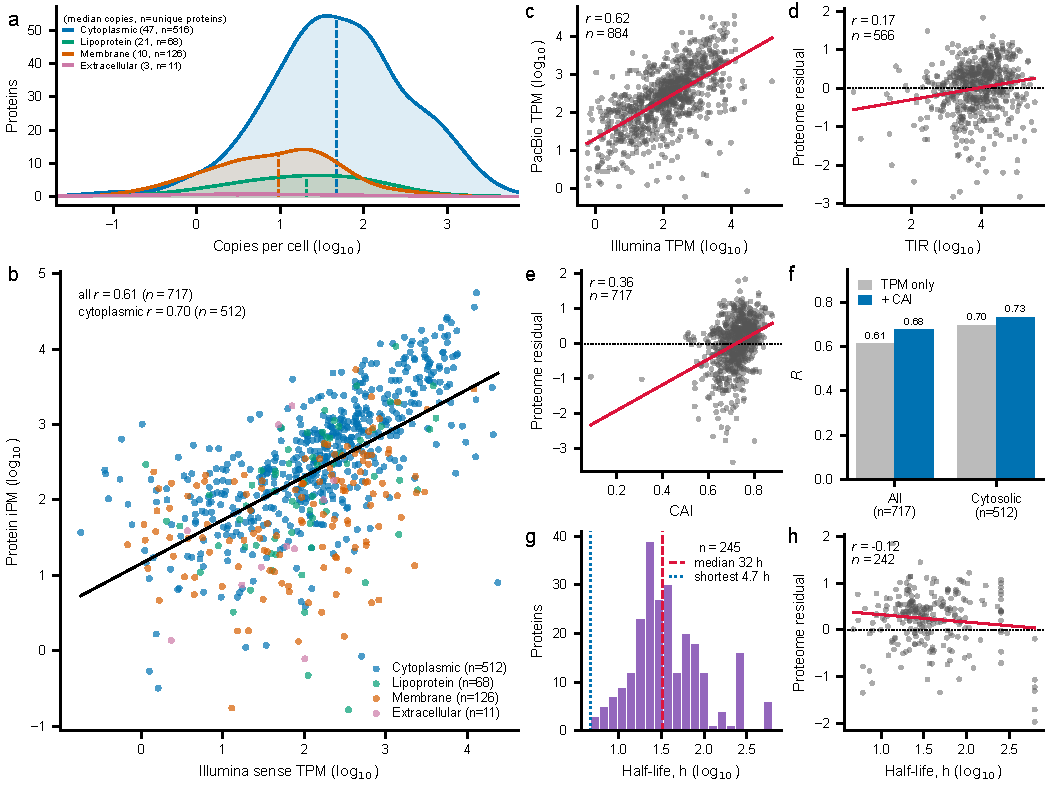
\includegraphics[scale=1]{figures/correlation.pdf}% born-at-size: render at native size (5.25 in), no scaling
    \caption{\textbf{Transcriptome--proteome correlation in \syn.}
    (a) Per-protein copy-number distribution by localization (cytoplasmic, lipoprotein, membrane, extracellular).
    (b) Illumina sense TPM versus proteome iPM ($\log_{10}$).
    (c) PacBio versus Illumina sense TPM ($\log_{10}$).
    (d) Model Pearson $R$ for the whole proteome and for cytoplasmic proteins, with and without CAI.
    (e) Intrinsic protein half-lives as protease degradation transferred from \mpn.}
	 \label{fig:correlation}
\end{figure}

\begin{sifigure}
    \centering
    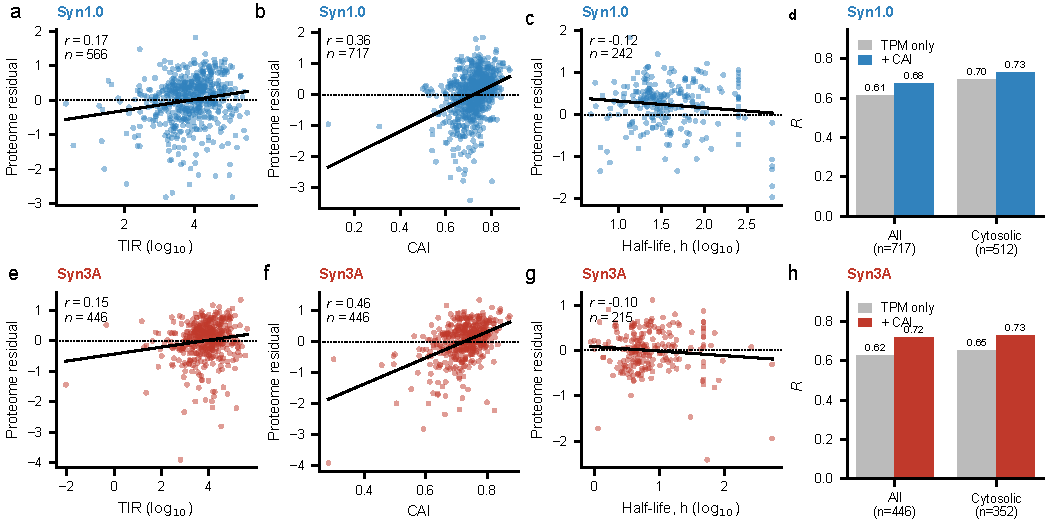
\includegraphics[scale=1]{figures/si-correlation.pdf}% born-at-size: native 177.8 mm, fits the 180 mm text block
    \caption{\textbf{Supporting transcriptome--proteome analysis for \syn~and \syna.}
    (a) Length dependence of the PacBio-to-Illumina sense-TPM ratio in \syn.
    (b) Abundance dependence of the same ratio (MA plot).
    (c) Predicted TIR versus the \syn~proteome residual.
    (d) CAI versus the \syn~proteome residual.
    (e) \syn~protein half-life versus the proteome residual.
    (f) \syna~per-protein copy-number distribution by localization.
    (g) \syna~Illumina sense TPM versus proteome iPM ($\log_{10}$).
    (h) \syna~predicted TIR versus the proteome residual.
    (i) \syna~CAI versus the proteome residual.
    (j) \syna~intrinsic protein half-lives transferred from \mpn.
    (k) \syna~protein half-life versus the proteome residual.
    (l) \syna~model Pearson $R$ for the whole proteome and for cytoplasmic proteins, with and without CAI.}
    \label{fig:si-correlation}
\end{sifigure}
